\subsection{Notacja Forsytha-Edwardsa}
\label{subsec:notacja-fen}


W 1950 roku amerykański matematyk Claude Shanon na łamach \("\)Philosophical Magazine\("\) opublikował pracę naukową zatytułowaną \("\)Programowanie komputera do gry w szachy\("\).~\cite*{Shannon1950XXIIPA}
Stała się ona teoretyczną podstawą dla dalszego rozwoju silników szachowych.
Zawarte w niej zostało między innymi oszacowanie, co do ilości możliwych pozycji szachowych, wynoszące~$10^{43}$.
Oznacza to, że liczba legalnych ułożeń planszy o rzędy wielkości przewyższa liczbę gwiazd w widzialnym wszechświecie.

Aby umożliwić użytkownikowi efektywne wprowadzenie danych oraz komunikację z~programem, należało w pierwszej kolejności sprecyzować format, w jakim zostaną dostarczone informacje dotyczące aktualnej pozycji.
Standardem, wykorzystywanym nie tylko w większości silników, ale także w pojedynkach rozgrywanych online, jest Notacja Forsytha-Edwardsa (ang.~\emph{Forsyth–Edwards~Notation}, w~skrócie FEN).

Notacja FEN jest sześciopolową linią znaków ASCII, która pozwala na precyzyjne określenie aktualnego stanu gry.
Wielkimi literami kodowane są bierki białe, małymi natomiast bierki czarne.
Każda z nich opisana jest skrótem pochodzącym od ich angielskich nazw.

%
%
%\begin{multicols}{3}
%    \begin{itemize}
%        \item P/p — pion
%        \item N/n — skoczek
%        \item B/b — goniec
%        \item R/r — wieża
%        \item Q/q — hetman
%        \item K/k — król
%    \end{itemize}
%\end{multicols}
%
%Sześć następujących po sobie pól, oddzielonych spacjami, określa kolejne aspekty gry:
%\begin{enumerate}[itemsep=0.3em]
%    \item Reprezentacja 64 pól szachownicy z perspektywy białego gracza.
%    Każdy z wierszy planszy oddzielony jest \("\)/\("\), a jego zawartość opisywana zostaje od kolumny a, do kolumny h.
%    Liczbę nieprzerwanie pustych pól w danym wierszu określa cyfra z zakresu od 1 do 8.
%    \item Sprecyzowanie, do którego gracza należy następny ruch (w - biały, b - czarny).
%    \item Przedstawienie możliwości roszady obu stron (K/k - krótka roszada, Q/q - długa roszada).
%    \item Sprecyzowanie pola będącego celem bicia w przelocie, szerzej znanego jako ruch en~passant.
%    Brak możliwości bicia określany jest jako\("\)-\("\)
%    \item Liczba posunięć od ostatniego bicia bądź ruchu pionem.
%    Wartość ta jest istotna z punktu widzenia reguły 50 posunięć.
%    \item Liczba pełnych ruchów, która zostaje każdorazowo zwiększana po ruchu czarnych bierek.
%\end{enumerate}

Pełna specyfikacja FEN dostępna jest w dokumentacji \("\)Portable Game Notation\("\). \cite*{PGNdoc}

\begin{figure}[ht]
    \centering
    \begin{tabular}{@{}ll@{}}
        a) & b) \\
        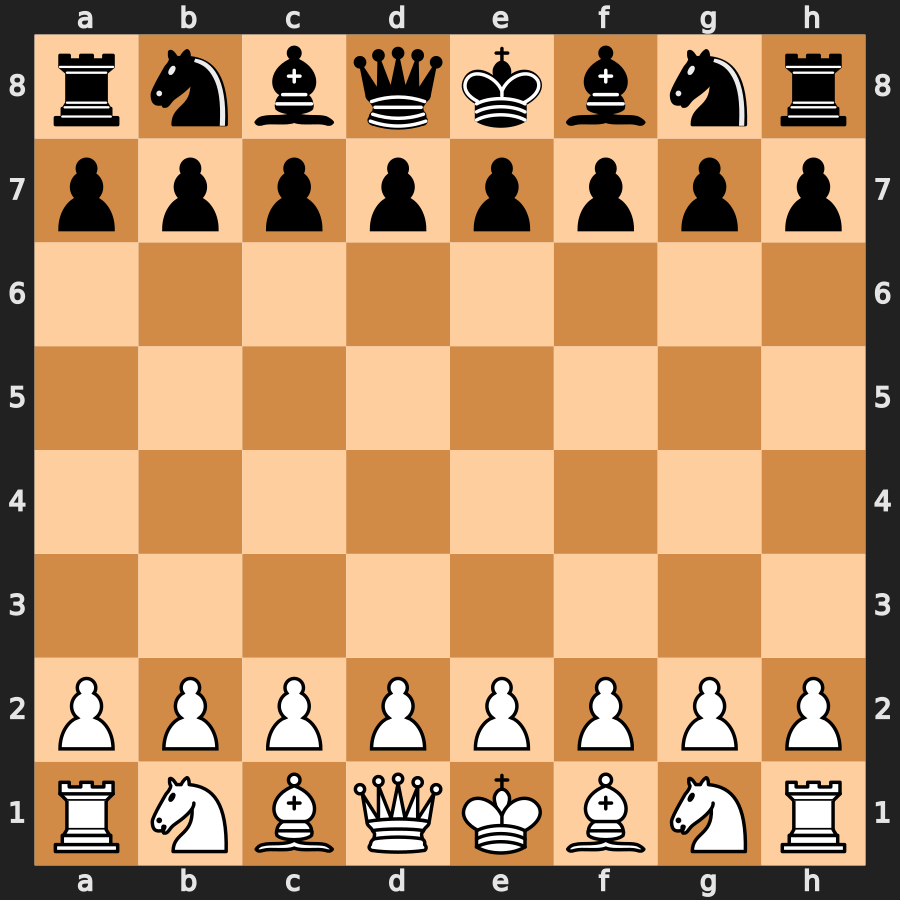
\includegraphics[width=0.35\textwidth]{rozdzialy/rozdzial01/1_komunikacja-z-systemem/rysunki/pozycja_startowa}
        &
        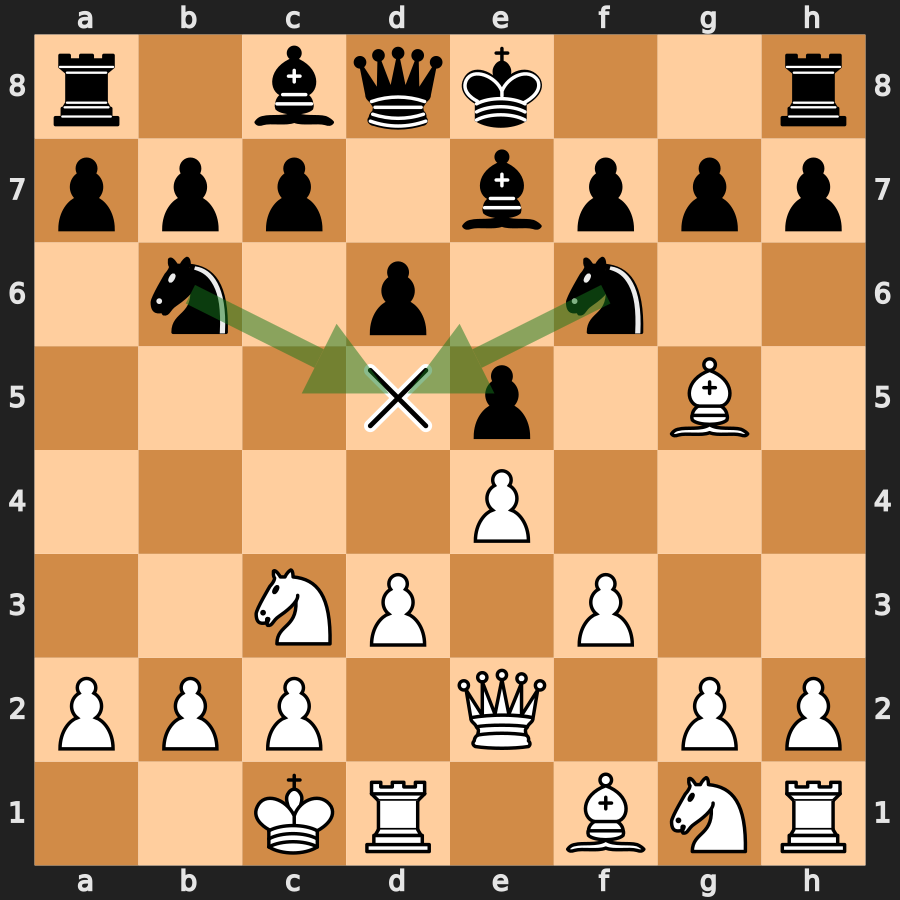
\includegraphics[width=0.35\textwidth]{rozdzialy/rozdzial01/1_komunikacja-z-systemem/rysunki/pozycja_niejasna}
    \end{tabular}
    \caption{Przykładowe pozycje szachowe: a) startowa, b) po paru ruchach}
    \label{fig: basic_chess_positions}
\end{figure}

\centerline{
    \ref{fig: basic_chess_positions} a) \lstset{basicstyle=\ttfamily}\lstinline{rnbqkbnr/pppppppp/8/8/8/8/PPPPPPPP/RNBQKBNR w KQkq - 0 1}
}
\centerline{
    \ref{fig: basic_chess_positions} b) \lstset{basicstyle=\ttfamily}\lstinline{r1bqk2r/ppp1bppp/1n1p1n2/4p1B1/4P3/2NP1P2/PPP1Q1PP/2KR1BNR b kq - 7 7}
}

